\chapter{Minimal problems in geometry of computer vision}\labelcha{app}
Many problems from geometry of computer vision can be modeled by systems of polynomial equations.
A problem that requires only the minimal subset of data points to solve the problem is called a minimal problem.
A typical example is the 5-point algorithm \cite{5pt} for relative pose estimation between two cameras given five image correspondences only.
In many applications, solvers of these minimal problems are used in the Random Sample Consensus (RANSAC) algorithm \cite{ransac}, where the minimal problems has to be solved repeatedly for a large amount of input data.
Thus, these solvers are required to be fast and efficient.
The state of the art method is to generate these solvers by automatic generators \cite{autogen, larsson}, which are based on Gr\"obner bases construction and eigenvectors of multiplication matrices computation.
In these solvers both real and non-real solutions are computed, but the non-real solutions are discarded, since they have no geometric meaning.

In \refsec{POP:sol}, we have proposed and implemented an algorithm, which does not need to compute the superfluous non-real solutions, and therefore may be faster than the standard solvers generated by the automatic generator.
In this section, we compare the speed and the numerical stability of the state of the art solvers with our implementations of the moment method algorithm for polynomial system solving.
For this reason, we have selected few minimal problems from geometry of computer vision, on which we will compare the selected solvers.

\section{Dataset description}
\input{macros/app_LADIO.tex}
First of all, we describe the scene, which we have chosen for our experiments.
It is a real scene of a sculpture of Buddha head taken for the LADIO \cite{ladio} project.
The reconstructed 3D model can be seen at webpage \url{https://skfb.ly/67ZxD} and the source images are publicly available at Github in repository \href{https://github.com/alicevision/dataset\_buddha}{\nolinkurl{alicevision/dataset\_buddha}}.
For the reader we show the reconstructed surface of the sculpture in \reffig{app:LADIO}.

\begin{figure}[ht]
  \centering
  \begin{subfigure}[b]{0.45\textwidth}
    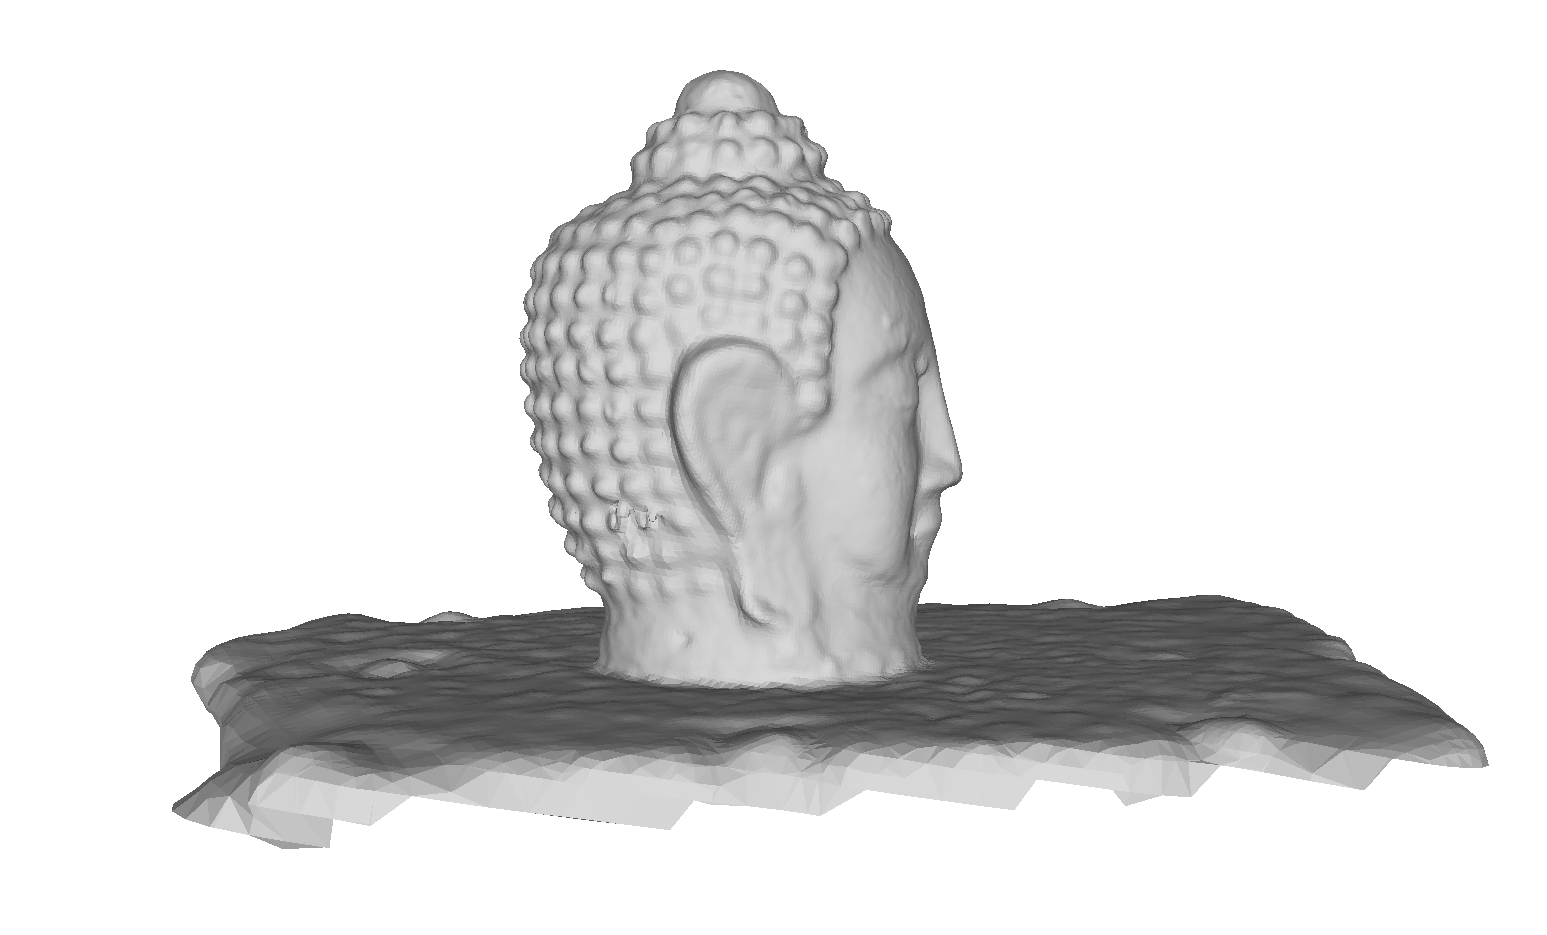
\includegraphics[width=0.95\textwidth]{images/LADIO_01.png}
    \vspace{2mm}
  \end{subfigure}
  ~
  \begin{subfigure}[b]{0.45\textwidth}
    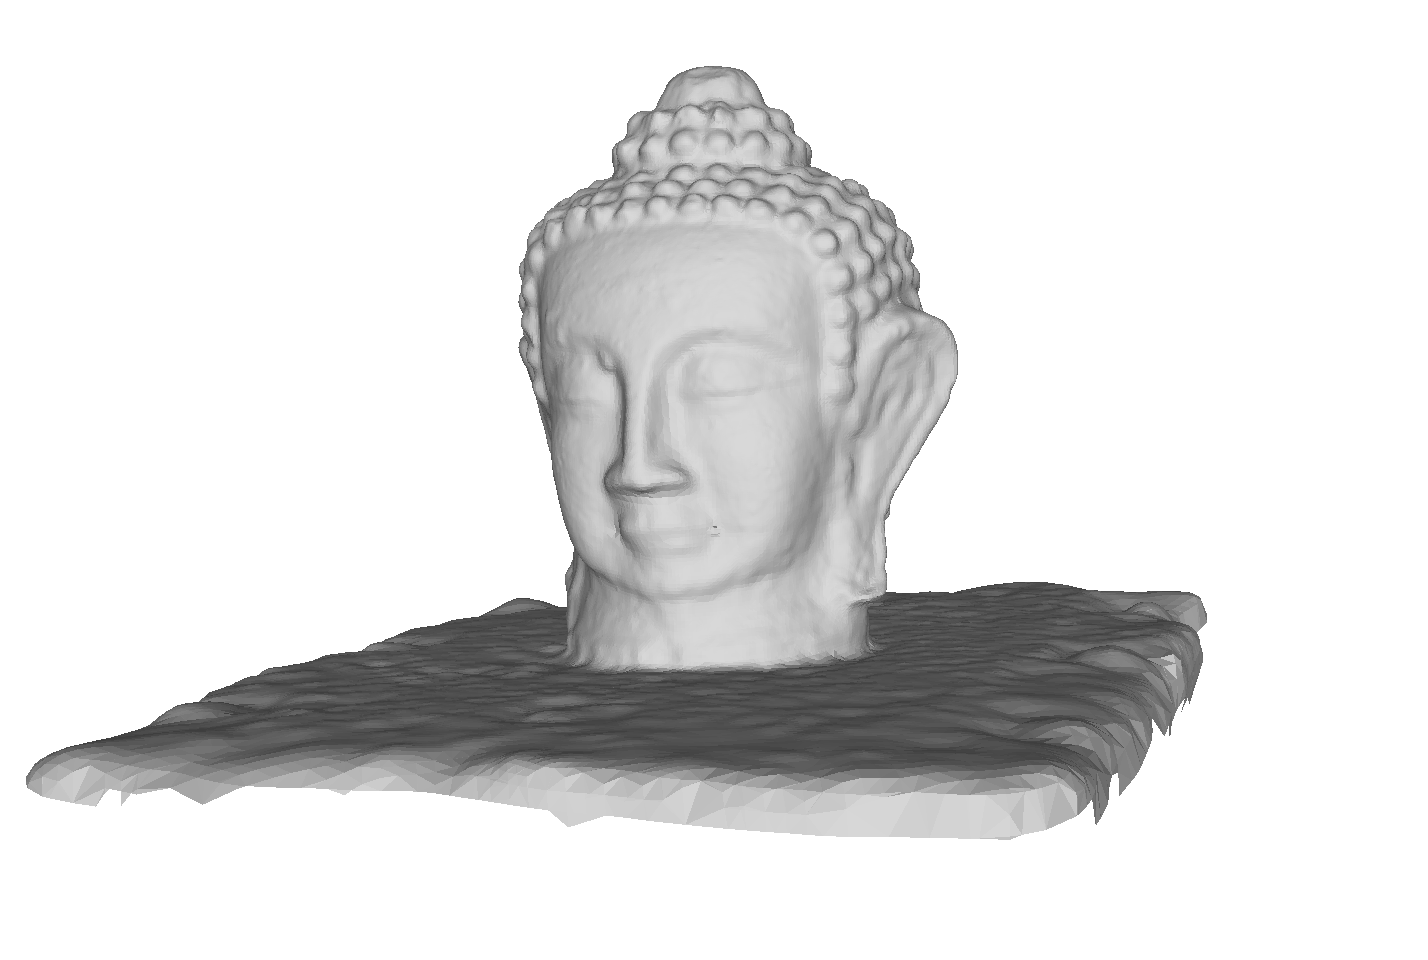
\includegraphics[width=0.90\textwidth]{images/LADIO_02.png}
  \end{subfigure}
  \caption{Sculpture of Buddha head. Surface representing a point cloud reconstructed from the taken images.}
  \labelfig{app:LADIO}
\end{figure}

There are \importAppLADIONumCameras{} taken images of the sculpture, from which \importAppLADIONumPoints{} spatial points were reconstructed using a scene reconstruction pipeline from the photogrammetric framework named Alice Vision \cite{ALiceVision}.
This complex pipeline consists of SIFT \cite{sift} feature detection, RANSAC \cite{ransac} outlier detection framework using epipolar geometry and incremental structure from motion (SfM) algorithm.
This algorithm starts with epipolar geometry between two cameras triangulating the corresponding 2D features into 3D points.
Then, new cameras are iteratively added and resectioned based on the 2D-to-3D correspondences using the perspective-n-point (PnP) \cite{pnp} algorithm in a RANSAC \cite{ransac} framework.
Pose of each added camera is then refined by a non-linear optimization.
After that new 3D points are triangulated and by a bundle adjustment (BA) extrinsic and intrinsic parameters of all cameras as well as the position of all 3D points are refined.
Then, next iteration of the SfM algorithm is performed until all cameras are estimated.
Next step of the reconstruction pipeline is the retrieval of the depth value for each pixel for each reconstructed cameras.
The method used in the pipeline is the semi-global matching (SGM) \cite{sgm} method.
After that mesh is created from the reconstructed point cloud by the 3D Delaunay tetrahedralization, which is then textured.

Usage this complex reconstruction pipeline provides us good ground truth values for our experiments with minimal number of outliers.

All the experiments were executed on Intel Xeon E5-1650 v4 CPU 3.60GHz based computer with sufficient amount of free system memory.
The installed version of Python was 3.5.3 and MATLAB R2017b 64-bit was used.

\section{Calibrated camera pose}
Computation of calibrated camera pose (its rotation and location with respect to the global coordinate system) is one of the typical problems in computer vision.
The pose can be computed from at least three known 3D points and their perspective projection into the image plane, thus the problem is called the perspective-three-point (P3P) problem and it is known since 1841 from \cite{p3p1841}, but its modern and complete description can be found in \cite{P3P}.

\begin{figure}[ht]
  \centering
  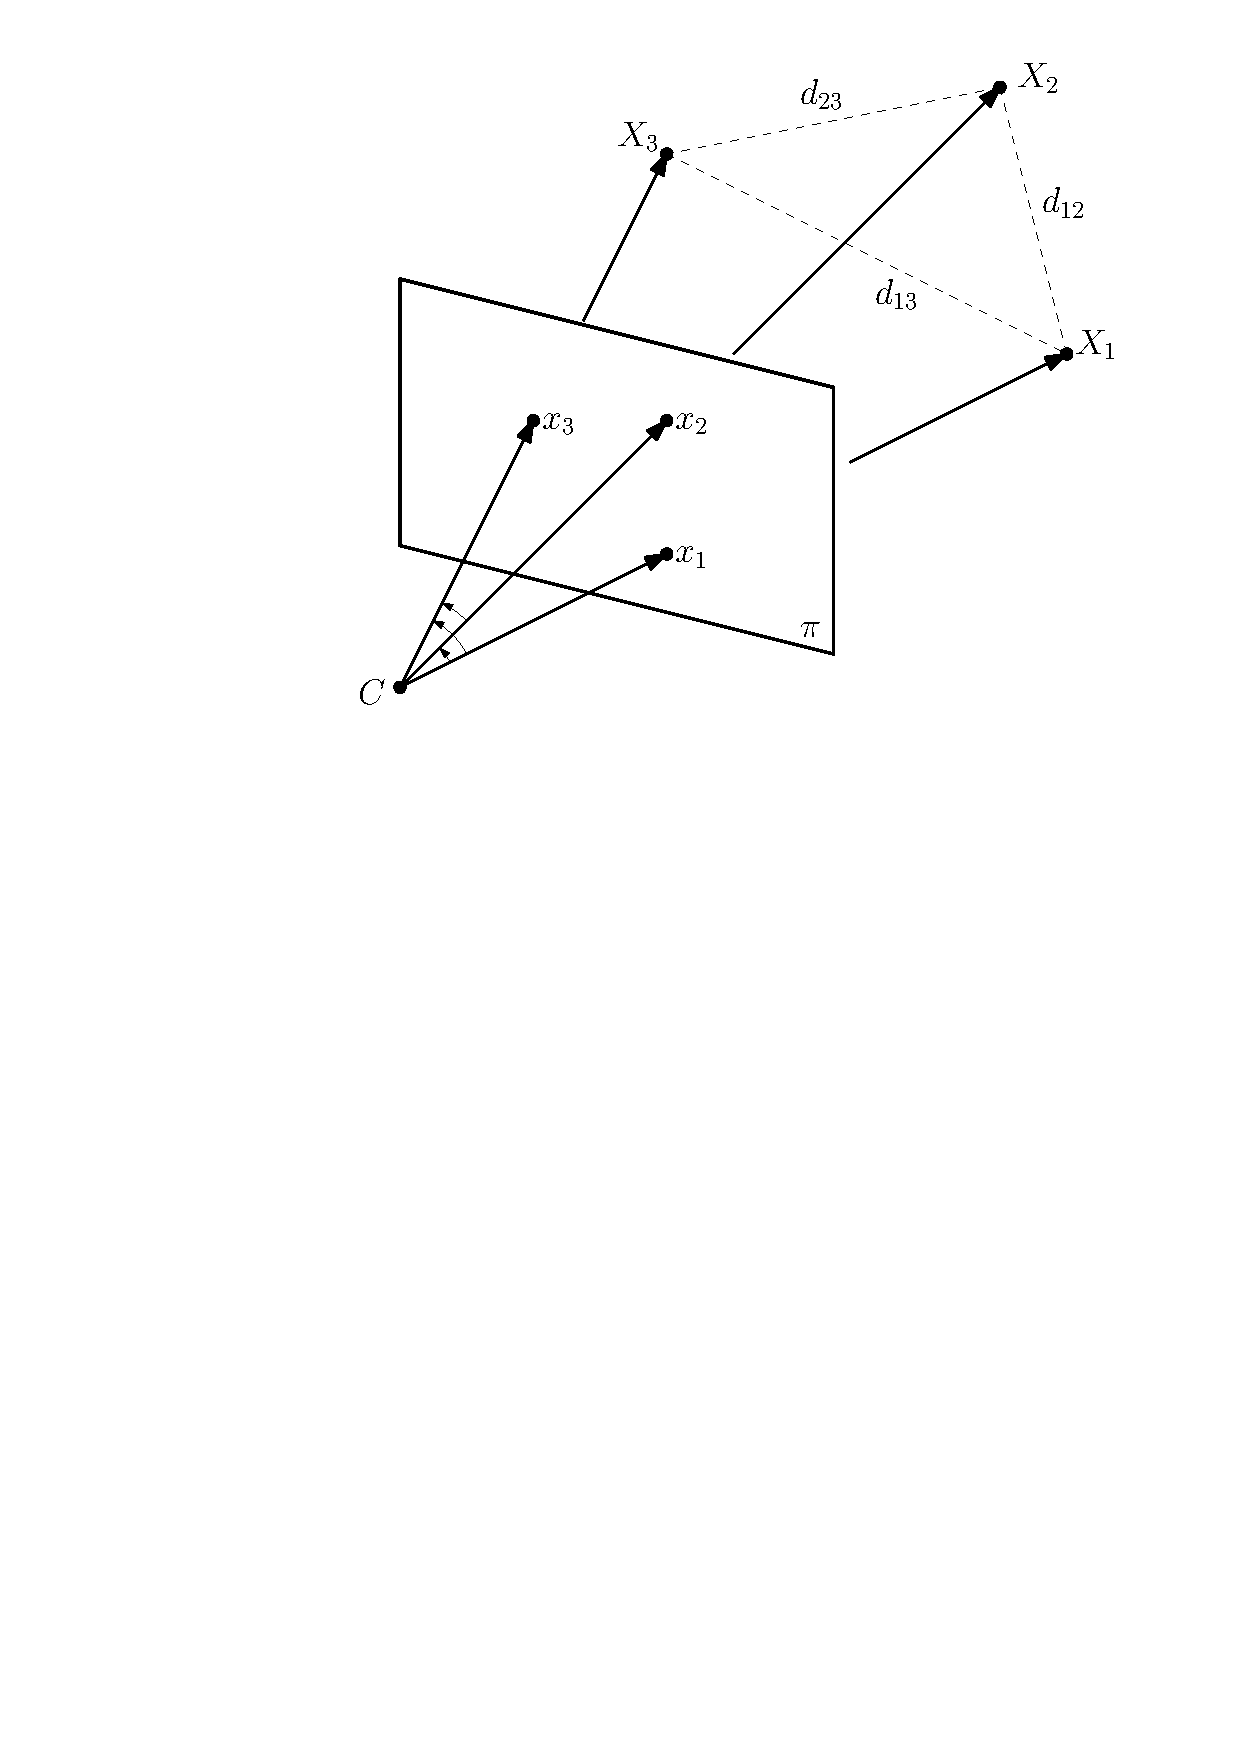
\includegraphics[width=0.5\textwidth]{drawings/P3P.pdf}
  \caption{Scheme of the P3P problem. A pose of a calibrated camera can be computed from three known 3D points $X_1$, $X_2$, $X_3$ and their projections $x_1$, $x_2$, $x_3$ into the image plane $\pi$. The camera projection center is denoted as $C$. Distances $d_{12}$, $d_{23}$, $d_{13}$ denote the distances between the respective 3D points.}
  \labelfig{app:P3P}
\end{figure}

The problem is stated followingly:
Given three 3D points $X_1, X_2, X_3 \in\R^3$ in the global coordinate system and their projections $x_1, x_2, x_3 \in\R^2$ respectively into the image plane in the image coordinate system, we are looking for a camera projection center position $C\in\R^3$ and a camera rotation matrix $R\in\SO$ -- all rotations in 3D space around the origin, such that the projection equation
\begin{align}
  \lambda_i\bmB x_i\\1\bmE &= K\bmB R & -RC\bmE\bmB X_i\\1\bmE
\end{align}
holds for $i=1,2,3$ and $\lambda_i\in\R/\{0\}$, where $K\in\R^{3\times3}$ is known calibration matrix of the camera.
The situation is depicted in \reffig{app:P3P}.

It has been shown that for a general case this problem can be solved by finding roots of a quartic equation in variable $\xi\in\R$
\begin{align}
  a_4\xi^4 + a_3\xi^3 + a_2\xi^2 + a_1\xi + a_0 &= 0\labeleq{app:P3P:4}
\end{align}
with coefficients $a_0, \ldots, a_4\in\R$, which can be computed by the formulae below.
\begin{align}
  a_4 &= -4d_{23}^4d_{12}^2d_{13}^2c_{23}^2+d_{23}^8-2d_{23}^6d_{12}^2-2d_{23}^6d_{13}^2+d_{23}^4d_{12}^4+2d_{23}^4d_{12}^2d_{13}^2+d_{23}^4d_{13}^4\\
  a_3 &= 8d_{23}^4d_{12}^2d_{13}^2c_{12}c_{23}^2+4d_{23}^6d_{12}^2c_{13}c_{23}-4d_{23}^4d_{12}^4c_{13}c_{23}+4d_{23}^4d_{12}^2d_{13}^2c_{13}c_{23}\\
      &-4d_{23}^8c_{12}+4d_{23}^6d_{12}^2c_{12}+8d_{23}^6d_{13}^2c_{12}-4d_{23}^4d_{12}^2d_{13}^2c_{12}-4d_{23}^4d_{13}^4c_{12}\nonumber\\
  a_2 &= -8d_{23}^6d_{12}^2c_{13}c_{12}c_{23}-8d_{23}^4d_{12}^2d_{13}^2c_{13}c_{12}c_{23}+4d_{23}^8c_{12}^2-4d_{23}^6d_{12}^2c_{13}^2\\
      &-8d_{23}^6d_{13}^2c_{12}^2+4d_{23}^4d_{12}^4c_{13}^2+4d_{23}^4d_{12}^4c_{23}^2-4d_{23}^4d_{12}^2d_{13}^2c_{23}^2+4d_{23}^4d_{13}^4c_{12}^2+2d_{23}^8\nonumber\\
      &-4d_{23}^6d_{13}^2-2d_{23}^4d_{12}^4+2d_{23}^4d_{13}^4\nonumber\\
  a_1 &= 8d_{23}^6d_{12}^2c_{13}^2c_{12}+4d_{23}^6d_{12}^2c_{13}c_{23}-4d_{23}^4d_{12}^4c_{13}c_{23}+4d_{23}^4d_{12}^2d_{13}^2c_{13}c_{23}-4d_{23}^8c_{12}\\
      &-4d_{23}^6d_{12}^2c_{12}+8d_{23}^6d_{13}^2c_{12}+4d_{23}^4d_{12}^2d_{13}^2c_{12}-4d_{23}^4d_{13}^4c_{12}\nonumber\\
  a_0 &= -4d_{23}^6d_{12}^2c_{13}^2+d_{23}^8-2d_{23}^4d_{12}^2d_{13}^2+2d_{23}^6d_{12}^2+d_{23}^4d_{13}^4+d_{23}^4d_{12}^4-2d_{23}^6d_{13}^2
\end{align}
Where the distances $d_{12}$, $d_{23}$ and $d_{13}$ are
\begin{align}
  d_{12} &= \|X_1 - X_2\|,\\
  d_{23} &= \|X_2 - X_3\|,\\
  d_{13} &= \|X_1 - X_3\|
\end{align}
and the coefficients $c_{12}$, $c_{23}$ and $c_{13}$ are cosines of the angles between the respective projection rays, and they can be directly computed from the projected points coordinates.
\begin{align}
  c_{12} &= \frac{x_1^\top K^{-\top} K^{-1}x_2}{\|K^{-1}x_1\|\|K^{-1}x_2\|}\\
  c_{23} &= \frac{x_2^\top K^{-\top} K^{-1}x_3}{\|K^{-1}x_2\|\|K^{-1}x_3\|}\\
  c_{13} &= \frac{x_1^\top K^{-\top} K^{-1}x_3}{\|K^{-1}x_1\|\|K^{-1}x_3\|}
\end{align}

The equation \refeqb{app:P3P:4} may have zero, two or four real roots, but some of them are discarded by checking three polynomial equations, that the law of cosines holds up to some numerical precision in triangles $\triangle\big(CX_iX_j\big)$ for $i,j=1,2,3$ and $i\neq j$, i.e.
\begin{align}
  d_{12}^2 &= \|X_1-C\|^2 + \|X_2-C\|^2 - 2c_{12}\|X_1-C\|\|X_2-C\|,\\
  d_{23}^2 &= \|X_2-C\|^2 + \|X_3-C\|^2 - 2c_{23}\|X_2-C\|\|X_3-C\|,\\
  d_{13}^2 &= \|X_1-C\|^2 + \|X_3-C\|^2 - 2c_{13}\|X_1-C\|\|X_3-C\|.
\end{align}
The camera pose ($C$ and $R$) is then computed from each of the remaining solutions.

The P3P problem is probably the simplest problem, which could be chosen from the geometry of computer vision for comparison of the polynomial systems solvers, since only one polynomial of degree four in one variable is given.

\input{macros/app_P3P.tex}
In the experiment, we have selected all available \importAppPPPNumCameras{} cameras, for each of them \importAppPPPNumPoints{} triplets of 2D--to--3D correspondences has been randomly chosen.
For each triplet, the coefficients $a_0, a_1, a_2, a_3, a_4$ of the equation \refeqb{app:P3P:4} has been precomputed.
Then, the real roots $\xi$  of the equation \refeqb{app:P3P:4} has been found by the selected polynomial solvers.
From $\xi$ the camera location $C$ and rotation $R$ has been computed in a standard way.
Then, the best tuple $C$ and $R$ minimizing the maximal reprojection error on all correspondences in the image for each camera and solver has been selected.

\subsection{Performance of the polynomial solvers}
We used the described P3P minimal problem to compare following polynomial systems solvers.
Firstly, we would like to see the performance of some state of the art purely algebraic solver.
A possible candidate is a solver generated by the automatic generator \cite{autogen}, which in case of one degree four polynomial equation in one variable is reduced to eigenvectors computation of multiplication matrix of size $4\times4$.
Secondly, the implementation of the moment method from the Polyopt package has been tested.
Thirdly, to be able to compare different implementations of the moment method with different implementation of the SDP solver, we have run the MATLAB implementation with MOSEK toolbox as described in \refsec{POP:sol:impl}.
Lastly, the MATLAB toolbox Gloptipoly \cite{gloptipoly} was used to compare the solvers with another method with built-in optimization.

The histograms of the maximal reprojection errors for the selected tuples of $C$ and $R$ for each polynomial solver can be seen in \reffig{app:P3P:histErr}.
For each estimated camera center position $C$, we have computed the error $e_C$ of the camera position compared to the ground truth values
\begin{align}
  e_C &= \|C-C_{GT}\|, \labeleq{app:P3P:CDist}
\end{align}
i.e.\ the distance of the estimated camera position to the ground truth position.
The histograms of these position errors for each polynomial solver are in \reffig{app:P3P:histCDist}.
For each estimated camera rotation $R$, we have computed the residual rotation to the ground truth camera rotation and computed the angle $e_R$ of this residual rotation as
\begin{align}
  e_R &= \arccos\bigg(\frac{1}{2}\Big(\tr\!\big(R_{GT}^{-1}R\big)-1\Big)\!\bigg). \labeleq{app:P3P:RAngle}
\end{align}
The histograms of the angles of residual rotations for each polynomial solver are in \reffig{app:P3P:histRAngle}.
We have also measured the execution time required to solve each instance of the equation \refeqb{app:P3P:4} by each polynomial solver and histogram of these times can be found in \reffig{app:P3P:histTimes}.
We have split the times to offline and online phases for the Polyopt package and the MATLAB implementation.
The offline phase is the part of the algorithm that does not depend on the given parameters of the problem but only on its structure, and therefore it can be precomputed in advance, as it is done in the automatic generator when generating the solver.
On the other hand, the online phase is dependent on the parameters, and thus it has be computed for each instance of the problem.
The performance of our implemented polynomial solvers depends on the number of iterations of \refalg{POP:sol:alg}.
This represents the variable $t$ from the algorithm, which is the degree of monomials, which are relaxed.
The values of $t$ at which the algorithm terminated are shown as histograms in \reffig{app:P3P:histRelax}.
For the Gloptipoly toolbox we have shown the values of two times the relaxation order, which has to be provided for the toolbox in advance.
This value is equivalent to the final value of the variable $t$.

\begin{figure}[ht]
  \centering
  \resizebox{0.95\textwidth}{!}{\input{graphs/app_P3P_err}}
  \caption{Histogram of the maximal reprojection errors of all correspondences in the image for the best camera positions and rotations estimated by the selected polynomial solvers for the P3P problem compared to the maximal reprojection errors computed for the ground truth camera positions and rotations.}
  \labelfig{app:P3P:histErr}
\end{figure}

\begin{figure}[ht]
  \centering
  \resizebox{0.95\textwidth}{!}{\input{graphs/app_P3P_cdist}}
  \caption{Histogram of the errors in estimated camera positions computed by the selected polynomial solvers for the P3P problem with respect to the ground truth camera positions.}
  \labelfig{app:P3P:histCDist}
\end{figure}

\begin{figure}[ht]
  \centering
  \resizebox{0.95\textwidth}{!}{\input{graphs/app_P3P_rangle}}
  \caption{Histogram of the errors in rotation angles computed by the selected polynomial solvers for the P3P problem with respect to the ground truth camera rotations.}
  \labelfig{app:P3P:histRAngle}
  %TODO: what about arccos(>1)
\end{figure}

\begin{figure}[ht]
  \centering
  \resizebox{0.95\textwidth}{!}{\input{graphs/app_P3P_times}}
  \caption{Histogram of the execution times required to compute the P3P problem by the selected polynomial solvers.}
  \labelfig{app:P3P:histTimes}
\end{figure}

\begin{figure}[ht]
  \centering
  \resizebox{0.95\textwidth}{!}{\input{graphs/app_P3P_relax}}
  \caption{Histogram of maximal degrees of relaxed monomials of the P3P problem. It corresponds to the value of variable $t$ in the last iteration of \refalg{POP:sol:alg} for the Polyopt package and the MATLAB with MOSEK implementation. For the Gloptipoly toolbox it corresponds to two times the given relaxation order.}
  \labelfig{app:P3P:histRelax}
\end{figure}

Further off, we are interested in the number of real solutions found by the polynomial solvers.
Since the algebraic solver computes all complex solutions first and then the non-real filters out, we are sure that this solver finds all real solutions.
On the other hand, given our observation, the methods based on optimization do not recover all real solutions, despite the theory.
The implementation from the Polyopt package has some numerical issues, which we were unable to remove in the time of writing this thesis, and therefore there is a small chance that the SDP solver fails in its computation and the solution is not found.
Moreover, the number of real solutions is related to the rank of the moment matrix found by the SDP solver, which  numerically depend on how good representative of the set $\K$ we have obtained.
This issue is common for both Polyopt implementation and the MATLAB with MOSEK implementation.
In case of the Gloptipoly toolbox, which is in the first case a polynomial optimization toolbox and not a polynomial system solver, the relaxation order has to be given in advance.
If the relaxation order is not high enough, no solution is found without distinguishing the cases when there is no solution or just the relaxation order is not high enough.
Surprisingly, when the relaxation order is too high, there are not found all the real solutions (typically one or none solution is found), because of reasons not known to us.
Therefore, we have set the relaxation order for Gloptipoly to one fixed value, in this case to three, which is the most common relaxation order from all runs of the Polyopt package and the MATLAB with MOSEK implementation, as you can see from \reffig{app:P3P:histRelax}.
Since these solvers are typically used in RANSAC-like \cite{ransac} algorithms, it may not be a big issue, when some of the real solutions are not found, of course depending the application.
For the reasons stated above we present in \reftab{app:P3P:numSol} number of all complex solutions and number of real solutions found by each of the polynomial solvers.

\begin{table}[ht]
  \centering
  \input{tables/app_P3P_numberSolutions.tex}
  \caption{Table of numbers of all real and complex solutions and of numbers of found real solutions by each of the selected polynomial solver for the P3P problem.}
  \labeltab{app:P3P:numSol}
\end{table}

We can see that for the P3P problem there is about $40$ \% of non-real solutions, which need not be computed.
We observe that in practice the moment method based implementations do not found all of the real solutions.
The Polyopt implementation found only $80$ \% of the solutions, but we belive that this can be improved up to $90$ \% success rate, which shows the MATLAB implementation.
Very poor results performed the Gloptipoly toolbox, but they can be probably improved by correct setting of the relaxation order.
On the other hand, from the histograms in Figures \reffignum{app:P3P:histErr}, \reffignum{app:P3P:histCDist}, \reffignum{app:P3P:histRAngle} we can see that the overall results for the P3P problem of the Polyopt implementation and the MATLAB implementation are comparable to the purely algebraic solver, despite they have not found all the real solutions.
Regarding the computation times shown in \reffig{app:P3P:histTimes}, we can see that the moment method based implementations are significantly slower than the  pure algebraic solver.
The best results from the moment method based solvers shows the Gloptipoly \cite{gloptipoly} toolbox, but note that we have set the relaxation order in advance, and therefore only one semidefinite program had to be solved for each instance.

\section{Calibrated camera pose with unknown focal length}
\input{macros/app_P35Pf.tex}
A computer vision problem slightly more complicated than the P3P problem is the calibrated camera pose estimation with unknown focal length.
In this problem the pose and focal length of a calibrated camera is estimated from four known 2D--to--3D correspondences.
This problem has seven degrees of freedom, and therefore is overconstrained with four points.
A minimal solver for this problem has been presented by C.~Wu in \cite{P35PfWu} using 3.5 points, i.e.\ ignoring one of the image coordinates for one of the points.
Since then, the problem is called the P3.5Pf problem.
However, this representation contains a degeneracy, which has been removed in \cite{P35Pf} by application of clever parametrization and clever elimination techniques.
We use this representation to test our implementations of the moment method.
The scheme of the problem geometry can be seen in \reffig{app:P35Pf}.

\begin{figure}[ht]
  \centering
  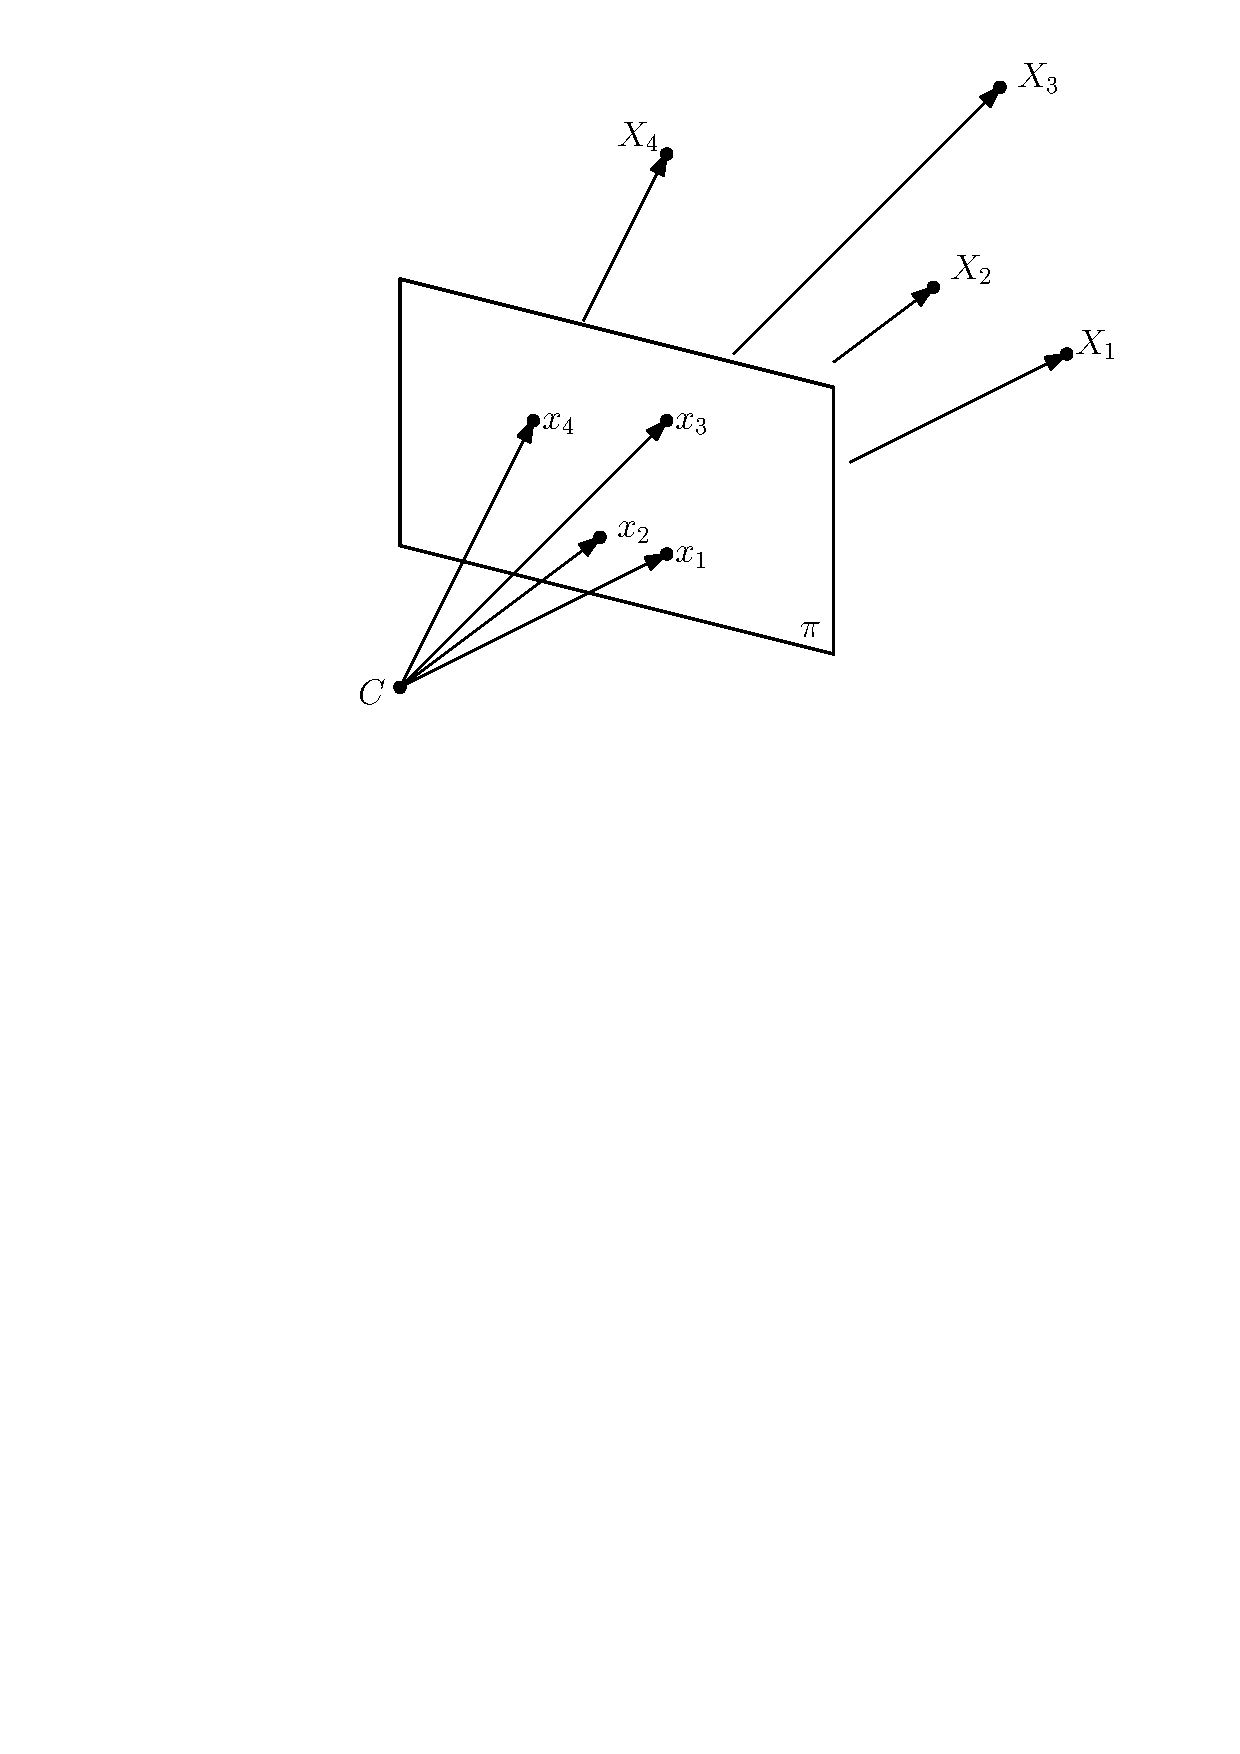
\includegraphics[width=0.5\textwidth]{drawings/P35Pf.pdf}
  \caption{Scheme of the P3.5Pf problem. A pose of a calibrated camera with unknown focal length can be computed from four known 3D points $X_1$, $X_2$, $X_3$, $X_4$ and their projections $x_1$, $x_2$, $x_3$, $x_4$ into the image plane $\pi$. The camera projection center is denoted as $C$.}
  \labelfig{app:P35Pf}
\end{figure}

The solution of the P3.5Pf problem comes from the projection equation
\begin{align}
  \lambda_i \bmB x_i\\ 1\bmE &= K_{known}K_f \bmB R & -RC\bmE \bmB X_i\\ 1 \bmE \labeleq{app:P35Pf:projection}
\end{align}
for $i = 1,2,3,4$ and $\lambda_i \in \R/\{0\}$, where $K_{known}\in\R^{3\times 3}$ is the known calibration matrix up to the unknown focal length, which is stored in the matrix $K_f = \diag\Big(\bmB f & f & 1\bmE^\top\Big)$.
The matrix $R\in\SO$ is the rotation matrix and the vector $C\in\R^3$ is the projection centre of the camera.
The 3D coordinates are given in vectors $X_i$ and their projections in vectors $x_i$.
We remove the known calibration matrix from the equation \refeqb{app:P35Pf:projection} by pre-calibrating of the image coordinates.
\begin{align}
  \tilde{x}_i &= K_{known}^{-1}x_i
\end{align}
We group the unknowns $f$, $R$ and $C$ into one camera projection matrix $P\in\R^{3\times4}$ as follows:
\begin{align}
  K_f \bmB R & -RC\bmE = P &= \bmB P_1^\top\\ P_2^\top\\ P_3^\top \bmE = \bmB p_{11} & p_{12} & p_{13} & p_{14}\\ p_{21} & p_{22} & p_{23} & p_{24}\\ p_{31} & p_{32} & p_{33} & p_{34}\bmE.\labeleq{app:P35Pf:P}
\end{align}
Then, the projection equation \refeqb{app:P35Pf:projection} is transformed into
\begin{align}
  \lambda_i \bmB \tilde{x}_i\\ 1\bmE &= P \bmB X_i\\ 1 \bmE.
\end{align}
Each 2D--to--3D correspondence gives us two linearly independent equations in the camera matrix.
\begin{align}
  P_1^\top \bmB X_i\\ 1\bmE - \tilde{x}_i\ind 1 P_3^\top \bmB X_i\\ 1 \bmE &= 0\\
  P_2^\top \bmB X_i\\ 1\bmE - \tilde{x}_i\ind 2 P_3^\top \bmB X_i\\ 1 \bmE &= 0
\end{align}
That gives us eight linearly independent equations and by ignoring one of them we get a minimal problem.
To fix the scale we add one additional equation
\begin{align}
  P_3^\top \bmB X_1\\ 1 \bmE &= 1.
\end{align}
These eight equations can be written in a matrix form
\begin{align}
  \bmB
    -X_1^\top & -1 & 0 & 0          & \tilde{x}_1\ind{1}X_1 & \tilde{x}_1\ind{1}\\
    0 & 0          & -X_1^\top & -1 & \tilde{x}_1\ind{2}X_1 & \tilde{x}_1\ind{2}\\
    -X_2^\top & -1 & 0 & 0          & \tilde{x}_2\ind{1}X_2 & \tilde{x}_2\ind{1}\\
    0 & 0          & -X_2^\top & -1 & \tilde{x}_2\ind{2}X_2 & \tilde{x}_2\ind{2}\\
    -X_3^\top & -1 & 0 & 0          & \tilde{x}_3\ind{1}X_3 & \tilde{x}_3\ind{1}\\
    0 & 0          & -X_3^\top & -1 & \tilde{x}_3\ind{2}X_3 & \tilde{x}_3\ind{2}\\
    -X_4^\top & -1 & 0 & 0          & \tilde{x}_4\ind{1}X_4 & \tilde{x}_4\ind{1}\\
    0 & 0          & 0 & 0          & X_1^\top & 1
  \bmE \bmB P_1\\ P_2\\ P_3 \bmE &= \bmB 0\\ 0\\ 0\\ 0\\ 0\\ 0\\ 0\\ 1 \bmE\\
  Ap &= b \labeleq{app:P35Pf:nullspace}
\end{align}
with coefficient matrix $A \in\R^{8\times 12}$ and vector $b \in\R^8$.
Then, we can parametrize the problem only by four unknowns using the vectors $p_1, p_2, p_3, p_4$ representing the nullspace of $A$ and particular solution $p_0$ of the equation \refeqb{app:P35Pf:nullspace}.
\begin{align}
  p &= p_0 + \xi_1p_1 + \xi_2p_2 + \xi_3p_3 + \xi_4p_4 \labeleq{app:P35Pf:subst}
\end{align}

To ensure that the camera projection matrix $P$ can be decomposed to $K_f$, $R$ and $C$ as stated in the equation \refeqb{app:P35Pf:P} we need to introduce next nine polynomial equations on $P$.
\begin{align}
  p_{21}p_{31} + p_{22}p_{32} + p_{23}p_{33} &= 0 \labeleq{app:P35Pf:eqs1}\\
  p_{11}p_{31} + p_{12}p_{32} + p_{13}p_{33} &= 0\\
  p_{11}p_{21} + p_{12}p_{22} + p_{13}p_{23} &= 0\\
  p_{11}^2 + p_{12}^2 + p_{13}^2 - p_{21}^2 - p_{22}^2 - p_{23} &= 0\\
  p_{13}^2p_{32} - p_{21}^2p_{32} - p_{22}^2p_{32} - p_{12}p_{13}p_{33} - p_{22}p_{23}p_{33} &= 0\\
  p_{12}p_{13}p_{32} + p_{22}p_{23}p_{32} - p_{12}^2p_{33} + p_{21}^2p_{33} + p_{23}^2p_{33} &= 0\\
  p_{11}p_{13}p_{32} + p_{21}p_{23}p_{32} - p_{11}p_{12}p_{33} - p_{21}p_{22}p_{33} &= 0\\
  p_{13}^2p_{31} - p_{22}^2p_{31} + p_{21}p_{22}p_{32} - p_{11}p_{13}p_{33} &= 0\\
  p_{12}p_{13}p_{31} + p_{22}p_{23}p_{31} - p_{11}p_{21}p_{33} - p_{21}p_{22}p_{33} &= 0 \labeleq{app:P35Pf:eqs9}
\end{align}
By solving these equations we obtain the unknowns $\xi_1, \xi_2, \xi_3, \xi_4$, from which we recover the projection matrix $P$, which we decompose by standard methods to $K_f$, $R$ and $C$.
In general the system of equations has 10 complex solutions.

In the experiment, we have randomly selected \importAppPPPfNumCameras{} cameras, for each of them \importAppPPPfNumPoints{} quadruples of 2D--to--3D correspondences has been randomly chosen.
For each quadruple, the coefficient vectors $p_0, p_1, p_2, p_3, p_4$ of the equation \refeqb{app:P35Pf:subst} has been precomputed.
Then, the real roots $\xi_1, \xi_2, \xi_3, \xi_4$ of the equations \refeqb{app:P35Pf:eqs1} -- \refeqb{app:P35Pf:eqs9} has been found by the selected polynomial solvers.
The focal length $f$, the camera location $C$ and the camera rotation $R$ has been computed in a standard way from the solutions.
Then, the best triple $f$, $C$ and $R$ minimizing the maximal reprojection error on all correspondences in the images for each camera and solver has been selected.

\subsection{Performance of the polynomial solvers}
We have tested our two implementations of the moment method, i.e.\ the Polyopt package and the MATLAB implementation with MOSEK semidefinite programming solver, on the previously described P3.5Pf problem.
We compared them with the state of the art polynomial solver Gloptipoly with fixed relaxation order to three and with a pure algebraic solver generated by the automatic generator \cite{autogen} as described in \cite{P35Pf}.
The generated solver consists of G-J elimination of a coefficient matrix of size $25 \times 35$ and of eigenvector computation of a multiplication matrix of size $10 \times 10$.

The histograms of the maximal reprojection errors can bee seen in \reffig{app:P35Pf:histErr}.
To evaluate the estimated focal length, we computed the relative focal length error for each of the estimated camera using the following formula:
\begin{align}
  e_f &= \bigg|\frac{f-f_{GT}}{f_{GT}}\bigg|.
\end{align}
The histograms of these relative focal length errors are shown in \reffig{app:P35Pf:histFRel}.
We have computed the errors in camera positions with respect to the ground truth values as described by the equation \refeqb{app:P3P:CDist}.
These errors are presented as histograms in \reffig{app:P35Pf:histCDist}.
Histograms of the residual rotation angle for each estimated camera computed by the equation \refeqb{app:P3P:RAngle} are in \reffig{app:P35Pf:histRAngle}.
Execution times required to solve each instance of the equations \refeqb{app:P35Pf:eqs1} -- \refeqb{app:P35Pf:eqs9} have been measured and presented in a form of histograms in \reffig{app:P35Pf:histTimes}.
Also the values of the variable $t$ from the last iteration of \refalg{POP:sol:alg} and the relaxation orders given to the Gloptipoly toolbox are shown as histograms in \reffig{app:P35Pf:histRelax}.
The numbers of all complex and real solutions as well as the numbers of found real solutions by each of the polynomial solver are written in \reftab{app:P35Pf:numSol}.

\begin{figure}[ht]
  \centering
  \resizebox{0.95\textwidth}{!}{\input{graphs/app_P35Pf_err}}
  \caption{Histogram of the maximal reprojection errors of all correspondences in the image for the best camera positions and rotations estimated by the selected polynomial solvers for the P3.5Pf problem compared to the maximal reprojection errors computed for the ground truth camera positions and rotations.}
  \labelfig{app:P35Pf:histErr}
\end{figure}

\begin{figure}[ht]
  \centering
  \resizebox{0.95\textwidth}{!}{\input{graphs/app_P35Pf_frel}}
  \caption{Histogram of the relative focal length errors computed by the selected polynomial solvers for the P3.5Pf problem with respect to the ground truth focal lengths.}
  \labelfig{app:P35Pf:histFRel}
\end{figure}

\begin{figure}[ht]
  \centering
  \resizebox{0.95\textwidth}{!}{\input{graphs/app_P35Pf_cdist}}
  \caption{Histogram of the errors in estimated camera positions computed by the selected polynomial solvers for the P3.5Pf problem with respect to the ground truth camera positions.}
  \labelfig{app:P35Pf:histCDist}
\end{figure}

\begin{figure}[ht]
  \centering
  \resizebox{0.95\textwidth}{!}{\input{graphs/app_P35Pf_rangle}}
  \caption{Histogram of the errors in rotation angles computed by the selected polynomial solvers for the P3.5Pf problem with respect to the ground truth camera rotations.}
  \labelfig{app:P35Pf:histRAngle}
  %TODO: what about arccos(>1)
\end{figure}

\begin{figure}[ht]
  \centering
  \resizebox{0.95\textwidth}{!}{\input{graphs/app_P35Pf_times}}
  \caption{Histogram of the execution times required to compute the P3.5Pf problem by the selected polynomial solvers.}
  \labelfig{app:P35Pf:histTimes}
\end{figure}

\begin{figure}[ht]
  \centering
  \resizebox{0.95\textwidth}{!}{\input{graphs/app_P35Pf_relax}}
  \caption{Histogram of maximal degrees of relaxed monomials of the P3.5Pf problem. It corresponds to the value of variable $t$ in the last iteration of \refalg{POP:sol:alg} for the Polyopt package and the MATLAB with MOSEK implementation. For the Gloptipoly toolbox it corresponds to two times the given relaxation order.}
  \labelfig{app:P35Pf:histRelax}
\end{figure}

\begin{table}[ht]
  \centering
  \input{tables/app_P35Pf_numberSolutions.tex}
  \caption{Table of numbers of all real and complex solutions and of numbers of found real solutions by each of the selected polynomial solver for the P3.5Pf problem.}
  \labeltab{app:P35Pf:numSol}
\end{table}

From the results of the polynomial solvers applied on the P3.5Pf problem we can see that there is only 50 \% of real solutions amongst all complex solutions.
Given efficient polynomial solver computing only real solutions, in theory we would be able to reduce the computation time to half in contrary to the state of the art algebraic solvers, which compute all complex solutions.
Although the moment based solvers did not recover all real solutions, the overall results are comparable to the algebraic solver as can be seen from the histograms.
The only disadvantage of the moment method based solvers is the computation time, which is incomparable to the algebraic solver.

\section{Conclusions}
We have described two minimal problems of computer vision: the calibrated camera pose problem and the calibrated camera pose with unknown focal length problem.
We have solved the polynomial systems arisen from these problems by our implementation of moment method in Python and MATLAB and compared it to Gloptipoly \cite{gloptipoly} toolbox and to algebraic solvers generated by the automatic generator \cite{autogen}.

Our implementation succeeded in solving these problems, which one them is one polynomial of degree four in one variable and the second one is a system of nine polynomials of degrees two and three in four variables.

The reprojection errors, errors in camera positions and rotations and the focal length relative errors of cameras estimated by the moment method are comparable to the errors of cameras estimated by the algebraic solvers.
On the other hand, the algebraic solvers are much faster than the implementations of the moment method.
